\documentclass[a4paper, oneside, 12pt, dvipdfmx]{book}

\usepackage[backend=biber,style=ieee]{biblatex}
\usepackage[dvipdfmx]{graphicx}
\usepackage{latexsym}
\usepackage{bmpsize}
\usepackage{booktabs}
\usepackage{siunitx}
\usepackage{url}
\usepackage{comment}
\usepackage{hyperref}
\usepackage[T1]{fontenc} %for polish alphabet
\usepackage{nameref} % for in-doc references | \labal{} |  \ref{}  \nameref{}
\usepackage{amsmath,amssymb} % for expectation sign
\usepackage[vlined, ruled]{algorithm2e}
\usepackage{amsmath,amssymb} % for expectation sign
\usepackage[vlined, ruled]{algorithm2e}


%% bibliography
\addbibresource{./src/bibliography.bib}


\begin{document}

%% use roman page numbering for abstract and acknowledgements
\pagenumbering{roman}

% \title{\bf{\LARGE{Sample of \LaTeX  Document} \\ \Large{\LaTeX のサンプルコード}}}
% \author{木幡咲希\\早稲田大学}
% \date{28年28月28日(Tsu)}
% \maketitle

\begin{titlepage}
\begin{center}
    \vspace{0.1\textheight}
    {\Large Bachelor Thesis 2023} \\
    \vspace{0.1\textheight}
    % \includegraphics[width=48truemm]{resources/0_title/waseda_logo.png} \\
    \vspace{0.05\textheight}
    \textbf{\huge Brush Style Transfer with \\ Feedforward Neural Networks} \\
    \vfill
    {\hspace{0.025\textwidth}\Large Supervisor \hspace{0.02\textwidth} Edgar Simo-Serra} \\
    {\Large Area of Study \hspace{0.02\textwidth} Computer Graphics} \\
    \vspace{0.05\textheight}
    {\Large Waseda University\\}
    \vspace{0.02\textheight}
    {\Large
        School of Fundamental Science and Engineering \\
        Department of Computer Science and Engineering \\}
    \vspace{0.05\textheight}
    {\Large 1W192140-3 Saki Kohata \\}
    \vspace{0.05\textheight}
    {Submitted on January 30, 2023}
\end{center}
\end{titlepage}

\cleardoublepage

%% abstract
\pagebreak
\hspace{0pt}
\vfill % magic commands to vertically center the content
    \begin{center}
        \textbf{Abstract}
    \end{center}
     Creating art used to require specialized knowledge and techniques for humans,
    but with the advancement of computer-generated art, many people can now create
    their own artworks. AI technology has also made it possible to transform 
    natural images into artistic style images, and there is also research on 
    transferring style from one image to another. However, when it comes to 
    creating tools to support creators, it is thought that transferring brush 
    styles, instead of the atmosphere of the painting, would be more effective. 
    In this paper, we adopt a Transformer-based model as a stroke prediction model 
    and attempted to generate strokes that imitate the brush style of a style 
    reference image. The generated images by the proposed model are not perfect 
    imitations of the brush style of the reference image. This is thought to be 
    caused by the limitation of the model to generate flexible strokes due to 
    minimal stroke parameters.

\vfill
\pagebreak

\pagebreak
\hspace{0pt}
\vfill % magic commands to vertically center the content
    \begin{center}
        \textbf{概要}
    \end{center}
     絵を描くことは専門的な知識や技術を必要としたが, CGアートの発達により多くの人が自らの手で
    作品を創り上げることが可能となった. また, AI技術の発達によって風景写真を芸術的なスタイルの
    画像に変換できるようになり, ある画像の全体的な雰囲気を別の画像に移す研究も既に行われている.
    しかし, クリエイターを支援するツールを作ることを考えると, 絵の全体的な雰囲気よりも, 絵を描
    く際に用いたブラシのスタイルを移すことに需要があると考えられる.
    本論文では, クリエイター支援ツールを作ることを目的に, スタイルの参照画像のブラシスタイルを
    模倣したストロークの生成タスクに取り組んだ. ブラシのストローク予測モデルには, Transformerを
    ベースとしたモデルを採用した.  提案モデルによる生成画像は参照画像のブラシスタイルを完全に
    模倣したものとはならなかった. これは, ストロークを表現するパラメータの数が最低限であること
    により, モデルの生成するストロークの表現力に限界があったことに起因するものだと考えられる.
\vfill
\pagebreak

%% acknowledgement
\pagebreak
\hspace{0pt}
\vfill 
    \begin{center}
    Acknowledgements
    \end{center}
     I am deeply grateful to my supervisor Edgar Simo-Serra, for his invaluable 
    guidance and support throughout my research. His insightful advice and assistance 
    have been invaluable in helping me complete this work.
    Also, I would like to extend my sincere appreciation to the members of my laboratory
    for their invaluable contributions to my research. Their insights and suggestions 
    during seminars and individual discussions have been instrumental in helping me 
    advance my work.
    I would also like to express my sincere appreciation to Kaishang Chen and  Yu Yanagida 
    for their invaluable help in providing templates and setting up the necessary 
    environment for me when I started working on this paper. 
    Lastly, I would like to express my heartfelt gratitude to my family and friends 
    who provided emotional support during this difficult time of the pandemic. 
    Their companionship and encouragement kept me going and helped me complete this work. 



\vfill
\pagebreak

%% use normal page numbering for the main body
\pagenumbering{arabic}

%% table of contents 
\tableofcontents
\listoffigures 
\listoftables

%% main body
\clearpage
\chapter{Introduction}
\section{Aim and Motivation}
 最後に書く!!!!!!
 


\section{Overview}
 This thesis consist of 6 chapters, including this introduction chapter Chapter 1.
In Chapter 2, we describe the various background knowledge and technologies that 
we draw upon in this paper, including a description of machine learning.
In Chapter 3, we introduce several papers that are related to our research.
In Chapter 4, we explain the proposed methodologies, and Chapter 5 details 
the experiment setup and presents the results.
Finally, in Chapter 6 we provide a summary of the main conclusions of 
the entire thesis.



\chapter{Background}
\section{Machine Learning}
\section{Neural Networks}
\section{Convolutional Neural Network}
\section{Transformers?}
\section{Autoencoders?} 
\chapter{Related Works}

\section{Image Style Transfer}
 Gatys \textit{et al}. \cite{Gatys_2016_CVPR} introduced \textit{A Neural Algorithm 
of Artistic Style} which enables the creation of novel images that seamlessly blend 
the subject matter of a photograph with the artistic style of a famous artwork.
In rendering the semantic content of an image in various styles, the problem was
the lack of effective image representations that can explicitly encode semantic 
information and separate image content and style. 
\textit{A Neural Algorithm of Artistic Style} \cite{Gatys_2016_CVPR} is able to 
analyze the visual characteristics of an image and separate them into two distinct 
components: the content and the style.
The content refers to the subject or object depicted in the image, while the style 
refers to the visual techniques manifested in a painting, such as touch and mood.

The algorithm in the paper uses a convolutional neural network (CNN) to extract
content and style features from two input images. The goal is to generate an 
output image that minimizes the difference between the content and style features 
of the input and output images, as measured by two loss functions defined in the 
paper. 

To minimize the difference in content features between the input and output images,
it is necessary to consider reducing the content loss function. 
Let $\vec{p}$ and $\vec{x}$ be the input image and the image that is generated by
the model, and  $P^l$ and $F^l$ be their feature representations of these images in 
layer l of the CNN. Then the loss function of the content of images is defined as:

\begin{equation}
    \label{contentloss}
    \mathcal{ L}_{content}(\vec{p}, \vec{x}, l)=\frac{1}{2} \sum_{i, j}\left(F_{i j}^l-P_{i j}^l\right)^2
\end{equation}
Similarly, to minimize the difference in style features between the input and
output images, we consider reducing the style loss function. The style of an 
image can be represented by the correlations of the outputs of the filters in 
each layer. This feature correlation is given by a Gram matrix, which is 
expressed as:
\begin{equation}
    G_{i j}^l = \sum_k F_{i k}^l F_{j k}^l 
\end{equation}
Let $\vec{a}$ and $\vec{x}$ be the input image and the image that is generated by
the model, and $A^l$ and $G^l$ be their style representations of these images in 
layer l of the CNN. The contribution of layer l to the total loss can be 
expressed as:
\begin{equation}
    E_l=\frac{1}{4 N_l^2 M_l^2} \sum_{i, j}\left(G_{i j}^l-A_{i j}^l\right)^2
\end{equation}
Based on this, we can define the loss function for the style of images as:
\begin{equation}
    \label{styleloss}
    \mathcal{ L}_{style}(\vec{a}, \vec{x})=\sum_{l=0}^\mathcal{ L}w_{l}E_{l}
\end{equation}
To transfer the style of image $\vec{a}$ to image $\vec{p}$, it is needed to 
create a new image that maintains the content representation of $\vec{p}$ 
while adopting the style representation of $\vec{a}$. To achieve this, we must 
minimize both Equation \ref{contentloss} and Equations \ref{styleloss}.
The final loss function to minimize is:

\begin{equation}
    \mathcal{ L}_{total}(\vec{p}, \vec{a}, \vec{x})=\alpha\mathcal{ L}_{content}(\vec{p}, \vec{x})+\beta\mathcal{ L}_{style}(\vec{a}, \vec{x})
\end{equation}


Figure \ref{output_IST} shows the images generated using this algorithm.
A is the original image, photo from Andreas Praefcke.
In the lower left corner of B through F, the paintings that provided the style 
for each of the generated images are shown.
B : \textit{The Shipwreck of the Minotaur} by J.M.W. Turner, 1805. 
C : \textit{The Starry Night} by Vincent van Gogh, 1889. 
D : \textit{Der Schrei} by Edvard Munch, 1893. 
E : \textit{Femme nue assise} by Pablo Picasso, 1910. 
F : \textit{Composition VII} by Wassily Kandinsky, 1913.

These are high quality paintings to which the style, such as the touch of the 
brush, has been adapted. 
However, the colors of the output picture are those of the style image, 
not the original image, and the result images have the characteristic objects of 
the style image (e.g., the moon, stars, and wavy clouds in \textit{The Starry Night}).
In this paper, we aim to address the problem of transferring only brush style 
in paintings.

\begin{figure}[p]
    \centering
    \includegraphics[width=130truemm]{resources/3_related_work/outputs_IST.png}
    \caption{
        Examples of images combining content and style, taken from
        \cite{Gatys_2016_CVPR}. 
    }
    \label{output_IST}
\end{figure}
\clearpage

\section{Machine painting like a human painter : DRL}
 Painting is a form of artistic expression that usually involving imaginative or 
creative skills, and it takes a lot of time and proper training to master the 
art.  Teaching a machine to paint is a challenging task, but researching it 
could lead to the development of tools that assist people in painting.

Huang \textit{et al}. \cite{Huang_2019_ICCV} trained a painting agent which 
imitates the painting process of humans. 
They employ a neural renderer in model-based deep reinforcement learning.
The agent is trained using model-based reinforcement learning, in which the 
agent learns to predict the outcomes of its actions and uses these predictions 
to plan its next actions, such as selecting a brush or color.
The agent is able to receive a larger reward as the visual quality of the 
paintings it create is better. The agent learns to make good painting choices by 
trying out various actions with the goal of maximizing the reward it receives.

It is demonstrated that their agent is able to learn to paint a variety of 
different styles and subjects, including handwritten digits, landscapes, 
portraits, and natural scene images. (Figure \ref{LearnToPaint})
\begin{figure}[h]
    \centering
    \includegraphics[width=120truemm]{resources/3_related_work/LearnToPaint.png}
    \caption{
        The painting results generated from the model introduced in the paper,
        taken from \cite{Huang_2019_ICCV}.
        (a) : MNIST dataset from \cite{deng2012mnist}. (b) SVHN dataset from \cite{netzer2011reading}.
        (c) : CelebA dataset from \cite{Liu_2015_ICCV}. 
        (d) : ImageNet dataset from \cite{russakovsky2015imagenet}.
    }
    \label{LearnToPaint}
\end{figure}
\newline
As shown in Figure \ref{LearnToPaint}, the model-based deep reinforcement 
learning method generates attractive paintings, but there seems to be problems
such as long training time for the agent and the instability of the agent.

\section{Machine painting like a human painter : FNNs}
 Liu \textit{et al}. \cite{liu2021paint} proposed Paint Transformer, a novel 
framework paintings from natural images by predicting parameters of multiple 
strokes without using reinforcement learning. 
Paint Transfer is a Transformer-based framework. This framework generates 
painting from natural images by using a feed-forward transformer to predict 
the multiple stroke parameters. 
Paint Transformer consists of two modules: the Stroke Predictor and the Stroke Renderer.  

In this work, strokes are represented by shape parameters ${x, y, h, w, \theta}$ 
and color parameters ${r, g, b}$.
\begin{figure}[h]
    \centering
    \includegraphics[width=110truemm]{resources/3_related_work/stroke-params.png}
    \caption{
        Parameter definition of a stroke,
        taken from \cite{liu2021paint}.
    }
    \label{strokeparams}
\end{figure}
\newline
The parameters are defined as shown in Figure \ref{strokeparams}, the center 
coordinates ($x$ and $y$), the height ($h$) and width ($w$) of the stroke, 
and the angle of rotation ($\theta$). Additionally, the RGB values of the 
stroke are represented by $r$, $g$, and $b$. Thus, the strokes generated are 
limited to monochromatic and linear.

Paint Transformer pipeline is shown in Figure \ref{PTpipeline}.
Stroke Predictor takes the target image It and the intermediate 
image $I_c$ as input, and generates a set of strokes $S_r$
(strictly speaking, it generates the parameters to determine the stroke set $S_r$).
The goal of training the Stroke Predictor is to make $S_r$ match a reference set
of strokes $S_f$. 
Stroke Renderer then takes each stroke in $S_r$ and generates a stroke image, 
which is combined with $I_c$ to create the final result image $I_r$.
This process can be expressed as follows:
\begin{equation}
    \label{painttransformer}
    I_r = PaintTransformer(I_c, I_t)
\end{equation}
\vspace{5mm}
\begin{figure}[t]
    \centering
    \includegraphics[width=150truemm]{resources/3_related_work/PTpipeline.png}
    \caption{
        A pipeline for Paint Transformer,
        taken from \cite{liu2021paint}.
    }
    \label{PTpipeline}
\end{figure}

\vspace{0.7cm}

\begin{figure}[h]
    \centering
    \includegraphics[width=150truemm]{resources/3_related_work/PTresult.png}
    \caption{
        The painting results generated from Paint Transformer,
        taken from \cite{liu2021paint}.
    }
    \label{PTresult}
\end{figure}
As shown in Figure \ref{PTresult}, this model produces highly quality paintings.
However, the strokes used are currently limited to monochromatic and linear forms.
To generate paintings with various touches, it should be explored more complex 
strokes with various shapes or color patterns.


\chapter{Methodology}

\section{Baseline}
 Our methodology is based on the \textit{"Paint Transformer: Feed Forward Neural Painting with Stroke Prediction"}
by Liu \textit{et al}. We selected Paint Transformer model for two main reasons. 
First, it has a self-learning stroke generation pipeline that does not require 
a pre-existing dataset of strokes, making it easy to train. Second, it uses 
FNNs rather than reinforcement learning, which allows for faster training and 
more stable models.
The Paint Transformer proposed in that paper is already briefly described in 
Chapter 3. The loss function used in that model is described in Section 4.4 
of this chapter. 
The model constructed by Liu \textit{et al} converts an input image into a 
picture-like image drawn by human strokes, but  we aim to address a different 
problem: transforming the content of the input image to match the style of a 
reference image. Specifically, we want to modify the content image such that 
it appears to have been painted with the same brushstrokes as the style image. 

\section{Network Structure}
 Our proposed model utilizes the same Stroke Predictor and Stroke Renderer 
as the baseline model.
A brief description of them was already given in Chapter 3, but we will explain
the Stroke Predictor in more detail.

As mentioned earlier in Chapter 3, the goal of the stroke predictor is to 
predict a set of strokes that don't differ from the reference stroke set. 
At the same time, it is also the goal of it that  to maintain a certain level
of abstraction to simulate the actual painting process.
As shown in Figure \ref{StrokePredictor}, Stroke Predictor uses a Transformer-based model 
that takes in two images: $I_c$ and $I_t$, and generates a stroke set through 
the use of two CNNs and a learnable positional encoding.
$F_c$ and  $F_t$, which are feature maps extracted from CNNs, and 
the encoding are concatenated and flattened as the input to the 
Transformer encoder. The decoder section uses $N$ learnable stroke 
query vectors as input. The output of the decoder consists of two 
branches of fully connected layers: one that predicts the initial 
stroke parameters, and another that predicts stroke confidence 
scores. The confidence scores are used to determine which predicted 
strokes should be plotted on the canvas. 
(For example, in Figure \ref{StrokePredictor}, confidence scores 
for the red, yellow and pink strokes are positive and only those 
are drawn on the canvas.)
During the backward phase of training, the sigmoid function is used 
to compute gradients in order to enable backpropagation.
\begin{figure}[h]
    \centering
    \includegraphics[width=110truemm]{resources/4_methods/StrokePredictor.pdf}
    \caption{
        Image of Stroke Predictor,
        taken from \cite{liu2021paint}.
    }
    \label{StrokePredictor}
\end{figure}

The baseline model takes an input image and generates a version of it that is 
represented as a series of brushstrokes.
However, we wanted to modify this process so that the content of 
the input image is transformed to match the style of a reference 
image, rather than just producing a stroke representation of the 
input image. To achieve this, we made changes to the process 
generating paintings from new images. 
The structure of our proposed model is shown in Figure \ref{Struct_ourmodel}.
The image $I_b$ is created from each base brush image, $G_g^b$ represents the 
gram matrix of $I_b$, and $G_r$ represents the gram matrix of the style 
reference image.

\begin{figure}[h]
    \centering
    \includegraphics[width=135truemm]{resources/4_methods/construct_ourmodel.pdf}
    \caption{
        The structure of our proposed model.
    }
    \label{Struct_ourmodel}
\end{figure}

The baseline provided one brush image, which was used to generate 
strokes by the Paint Transformer model. 
We expanded on this by creating multiple brush images and running 
the Paint Transformer model multiple times to generate pictures 
that depict the content of the input image using each brush image.
We then compared the style of the generated pictures to the style 
of the style reference image and selected the one with the 
smallest loss as the final output image. 

\section{Brush Images}
 Brush images used by the baseline model and created by us are shown in Figure \ref{Brushes}.
(a) is the brush image used by the baseline model, which is a pair of vertical and 
horizontal strokes. 
(b) and (c) are pairs of vertical and horizontal strokes, as was the baseline, 
and subsequent brush images are composed of a single image.
\begin{figure}[h]
    \centering
    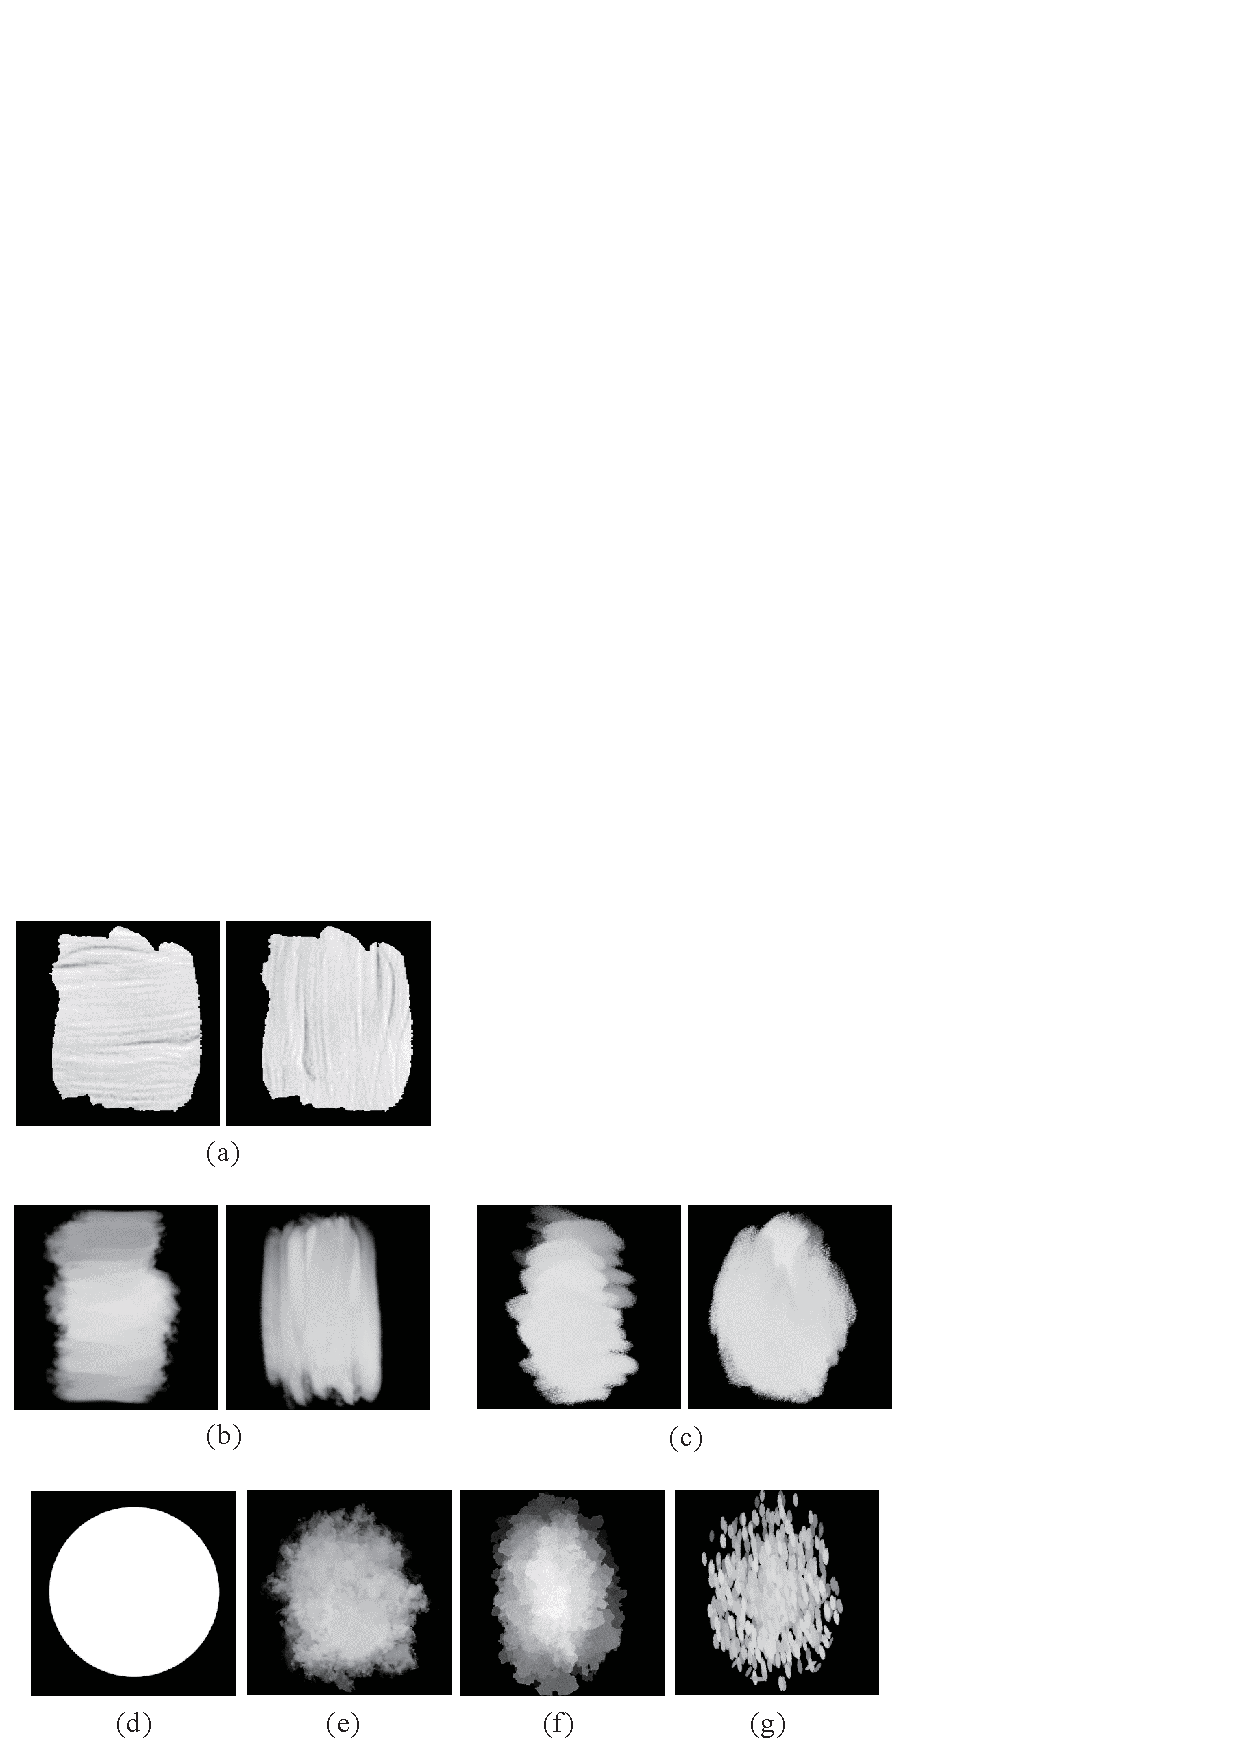
\includegraphics[width=130truemm]{resources/4_methods/brushes.pdf}
    \caption{
        Diversity of brushes developed for more accurate representation of painting effects.
    }
    \label{Brushes}
\end{figure}

\section{Loss Function}
 Since we are using the Paint Transformer proposed by Liu \textit{et al}, 
we also use loss functions proposed by them. However, we did not provide a 
detailed explanation of the loss functions in Chapter 3, so we will discuss 
them first. We will then describe the loss function we propose to measure 
the similarity of brush styles.

Paint Transformer considers loss functions at both the image level and the 
stroke level, and it introduces pixel loss, measurement of differences between
strokes, and stroke loss.
Pixel loss is a measure of the difference between the output image $I_r$ produced 
by the model and the target image $I_t$, which penalized on the image level.
It is expressed as :
\begin{equation}
    \mathcal{L}_{\text {pixel }}=\left\|I_r-I_t\right\|_1
\end{equation}
To measure the difference between two strokes, the L1 distance between two 
strokes, which is a measure of the difference between the parameters of the 
strokes, is defined. (Equation \eqref{L1-distance})
\begin{equation}
    \label{L1-distance}
    \mathcal{D}_{L_1}^{u, v}=\left\|s_u-s_v\right\|_1
\end{equation}
where $s_u$ and $s_v$ denote parameters of strokes u and v respectively. 
However, this measure does not take into account the different scales of 
big and small strokes, so the Wasserstein distance between the strokes is also 
included. The Wasserstein distance is calculated using the Gaussian distributions
of the strokes. 
A rotational rectangular stroke with brush shape parameters ${x, y, w, h, \theta}$
can be regarded as a two-dimensional Gaussian distribution $N(\mu, \sum)$ by the 
Equation \eqref{2D-GD}, and the Wasserstein Distance between two Gaussian 
distributions $N(\mu_u, \sum_u)$ and $N(\mu_v, \sum_v)$ can be expressed as in 
Equation \eqref{Wasserstein}.
\begin{equation}
    \label{2D-GD}
    \begin{aligned} \mu & =(x, y) \\ \boldsymbol{\Sigma}^{\frac{1}{2}} & =\left[\begin{array}{cc}\cos \theta & -\sin \theta \\ \sin \theta & \cos \theta\end{array}\right]\left[\begin{array}{cc}\frac{w}{2} & 0 \\ 0 & \frac{h}{2}\end{array}\right]\left[\begin{array}{cc}\cos \theta & \sin \theta \\ -\sin \theta & \cos \theta\end{array}\right] \\ & =\left[\begin{array}{cc}\frac{w}{2} \cos ^2 \theta+\frac{h}{2} \sin ^2 \theta & \frac{w-h}{2} \cos \theta \sin \theta \\ \frac{w-h}{2} \cos \theta \sin \theta & \frac{w}{2} \sin ^2 \theta+\frac{h}{2} \cos ^2 \theta\end{array}\right]\end{aligned}
\end{equation}
\begin{equation}
    \label{Wasserstein}
    \mathcal{D}_W^{u, v}=\left\|\mu_u-\mu_v\right\|_2^2+\operatorname{Tr}\left(\boldsymbol{\Sigma}_u+\boldsymbol{\Sigma}_v-2\left(\boldsymbol{\Sigma}_u^{\frac{2}{2}} \boldsymbol{\Sigma}_v \boldsymbol{\Sigma}_u^{\frac{1}{2}}\right)^{\frac{1}{2}}\right)
\end{equation}
Additionally, binary cross entropy (Equation \eqref{bce}) is used to match the confidence of the
predicted strokes with their ground truth labels. 
For a predicted stroke $s_u$ with confidence $c_u$ and a target stroke $s_v$ 
with ground truth label $g_v$,  $g_v$ will be equal to 1 if $s_v$ is a valid 
stroke, and $g_v$ will be equal to 0 if $s_v$ is an empty stroke.
\begin{equation}
    \label{bce}
    \mathcal{D}_{b c e}^{u, v}=-\lambda_r \cdot g_v \cdot \log \sigma\left(c_u\right)-\left(1-g_v\right) \cdot \log \left(1-\sigma\left(c_u\right)\right)
\end{equation}
where $\lambda_r$ is a weight term which controls the recall.
For strokes $s_u$ and $s_v$, their cost value is:
\begin{equation}
    M_{u, v}=g_v\left(\mathcal{D}_{L_1}^{u, v}+\mathcal{D}_W^{u, v}+\mathcal{D}_{b c e}^{u, v}\right)
\end{equation}
This function means the matching cost for empty target strokes is always 0.
Therefore, if the optimal permutations of the predicted and target strokes are $X$ and $Y$, 
respectively, the stroke loss function is defined as the sum of these costs, 
weighted by the weight terms  $\lambda_{L1}, \lambda_W$, and $\lambda_{bce}$.
\begin{equation}
    \begin{gathered}
        \mathcal{L}_{\text {stroke }}=\frac{1}{n} \sum_{i=1}^n\left(g_{Y_i}\left(\lambda_{L_1} \mathcal{D}_{L_1}^{X_i Y_i}+\lambda_W \mathcal{D}_W^{X_i Y_i}\right)\right.
        \left.+\lambda_{b c e} \mathcal{D}_{b c e}^{X_i Y_i}\right)
        \end{gathered}
\end{equation}

We adopted the $L1$ loss of the Gram matrix (Equation \eqref{gram}) as a loss function for measuring 
the similarity of brush styles.
By using the Gram matrix, it is possible to consider features over a wide range 
of positions, and we considered it to be effective for dealing with brush styles.



\chapter{Experiments and Results}

\section{Experimental Settings}
 Our experiments are conducted using the environment shown in Table \ref{environment}.

\setlength{\tabcolsep}{6pt}
\begin{table*}[h]
\begin{center} 
\caption{Environment of experiments}
\label{environment}
{\normalsize
\begin{tabular}{l c}

% content goes here
\toprule
Device & Available resources \\
\midrule
CPU & Intel(R) Xeon(R) E5-2690v4 CPU (2.60GHz)\\
Memory size & DDR4-2400 Reg.ECC 32GB\\
GPU & GeForce GTX 1080Ti  \\
\bottomrule
\end{tabular}
} \end{center} \end{table*}
\setlength{\tabcolsep}{6pt}


\section{Experiments}
 The model takes a content image and a style image and outputs a result image.
For the content images, we used one cat and one dog image from \textit{The Oxford-IIIT Pet Dataset}
\cite{Oxford-data} .
The content images and style images we used are shown in Figure \ref{dataset}.
\begin{figure}[h]
    \centering
    \includegraphics[width=115truemm]{resources/5_e_and_r/dataset.pdf}
    \caption{
        Content images and style images.
    }
    \label{dataset}
\end{figure}
Image (c) is \textit{Piet Mondrian Composition with Red, Blue, and Yellow}
by Piet Mondrian, 1930.
Image (d) is \textit{The Starry Night} by Vincent van Gogh, 1889. 

\vspace{3cm}
\section{Results}
 The output images obtained when painting the images (a) and (b) in Figure \ref{dataset} 
using all the brushes shown in Figure \ref{Brushes} are shown in Figure \ref{results}.
Images (a) to (g) in Figure \ref{results} correspond to brushes (a) to (g) in Figure \ref{Brushes}.
When we set images (c) and (d) in Figure \ref{dataset} as input to this 
model as style images, the images selected as output were images (d) and (e) 
in Figure \ref{results}, respectively.
This means that the brush style of image (c) in Figure \ref{dataset} and image 
(d) in Figure \ref{results} are considered similar. The same is true for image 
(d) in Figure \ref{dataset} and image (e) in Figure \ref{results}.
For clarity, the style reference image and the resulting image are shown side 
by side in Figure \ref{compare}.

 The generated image does not perfectly mimic the brush style of the reference 
image. 
It is considered that this is attributed to the fact that there are only seven 
base brushes and a minimal number of parameters to represent strokes.

\begin{figure}[p]
    \centering
    \includegraphics[width=90truemm]{resources/5_e_and_r/results.pdf}
    \caption{
        The output images.
    }
    \label{results}
\end{figure}

\begin{figure}[h]
    \centering
    \includegraphics[width=130truemm]{resources/5_e_and_r/compare.pdf}
    \caption{
        The style reference images input to our model and the resulting 
        images generated by the model.
    }
    \label{compare}
\end{figure}
\chapter{Discussions}

ブラシ画像は同じ画像をひっぱってつくられているけど、同じ画像の繰り返しにする
パターンもあって良いと思う。(クリスタのブラシで例を見せる)

\printbibliography

\end{document}
